\documentclass[DIV=calc, paper=a4, fontsize=11pt, twocolumn]{scrartcl}	 % A4 paper and 11pt font size
\usepackage[utf8]{inputenc}
\usepackage{lipsum} % Used for inserting dummy 'Lorem ipsum' text into the template
\usepackage[english]{babel} % English language/hyphenation
\usepackage[protrusion=true,expansion=true]{microtype} % Better typography
\usepackage{amsmath,amsfonts,amsthm} % Math packages
\usepackage[svgnames]{xcolor} % Enabling colors by their 'svgnames'
\usepackage[hang, small,labelfont=bf,up,textfont=it,up]{caption} % Custom captions under/above floats in tables or figures
\usepackage{booktabs} % Horizontal rules in tables
\usepackage{fix-cm}	 % Custom font sizes - used for the initial letter in the document

\usepackage{sectsty} % Enables custom section titles
\allsectionsfont{\usefont{OT1}{phv}{b}{n}} % Change the font of all section commands

\usepackage{fancyhdr} % Needed to define custom headers/footers
\pagestyle{fancy} % Enables the custom headers/footers
\usepackage{lastpage} % Used to determine the number of pages in the document (for "Page X of Total")

% Headers - all currently empty
\lhead{}
\chead{}
\rhead{}

% Footers
\lfoot{}
\cfoot{}
\rfoot{\footnotesize Page \thepage\ of \pageref{LastPage}} % "Page 1 of 2"

\renewcommand{\headrulewidth}{0.0pt} % No header rule
\renewcommand{\footrulewidth}{0.4pt} % Thin footer rule

\usepackage{lettrine} % Package to accentuate the first letter of the text
\newcommand{\initial}[1]{ % Defines the command and style for the first letter
\lettrine[lines=3,lhang=0.3,nindent=0em]{
\color{DarkGoldenrod}
{\textsf{#1}}}{}}

%----------------------------------------------------------------------------------------
%	TITLE SECTION
%----------------------------------------------------------------------------------------

\usepackage{titling} % Allows custom title configuration

\newcommand{\HorRule}{\color{DarkGoldenrod} \rule{\linewidth}{1pt}} % Defines the gold horizontal rule around the title

\pretitle{\vspace{-30pt} \begin{flushleft} \HorRule \fontsize{50}{50} \usefont{OT1}{phv}{b}{n} \color{DarkRed} \selectfont} % Horizontal rule before the title

\title{} % Your article title

\posttitle{\par\end{flushleft}\vskip 0.5em} % Whitespace under the title

\preauthor{\begin{flushleft}\large \lineskip 0.5em \usefont{OT1}{phv}{b}{sl} \color{DarkRed}} % Author font configuration

\author{Cristobal Donoso Oliva, Matias Medina Silva} % Your name

\postauthor{\footnotesize \usefont{OT1}{phv}{m}{sl} \color{Black} % Configuration for the institution name
Universidad de Concepción, CHILE % Your institution

\par\end{flushleft}\HorRule} % Horizontal rule after the title

\date{} % Add a date here if you would like one to appear underneath the title block

%----------------------------------------------------------------------------------------

\usepackage{graphicx}
\begin{document}

\maketitle % Print the title

\thispagestyle{fancy} % Enabling the custom headers/footers for the first page 

%----------------------------------------------------------------------------------------
%	ABSTRACT
%----------------------------------------------------------------------------------------

% The first character should be within \initial{}
\initial{E}\textbf{n el presente articulo se dispone al lector una instroducción a la teoría del caos aplicado a algorítmos bio-inspirados y blabla...}

%----------------------------------------------------------------------------------------
%	ARTICLE CONTENTS
%----------------------------------------------------------------------------------------

\section*{Introducción}
La ciencia en los sistemas físicos podríamos entenderla como un conjunto de reglas definidas y listas para ser utilizadas en estudios que desarrollan una evolución. Dicho de otra forma, sabemos que de manera determinística y en base a las leyes de la física newtoniana, podemos describir el comportamiento de muchos fenómenos físicos cotidianos. Sin embargo, muchos sistemas en la naturaleza son variables, sensibles a pequeñas perturbaciones en su entorno, o mejor dicho a las interacciones entre unidades básicas concordantes.\\\\La teoría del caos intenta explicar como evolucionan estos \emph{sistemas complejos}, estudiando el comportamiento de sistemas dinámicos que responden exageradamente desde condiciones iniciales. Un ejemplo conocido es el \emph{efecto mariposa} introducido por Edward Lorenz, el cual explica que pequeñas causas pueden tener grandes efectos.\\\\Los seres vivos se caracterizan por organizarse en estructuras complejas. A diario resuelven problemas mediante métodos colaborativos o competitivos, y en ésto radica la creación de algorítmos bio-inspirados.\\\\Con propósitos académicos demostrativos tomaremos de ejemplo a las bacterias. Estos organismos trabajan bajo el paradigma de la colaboración. En una población de bacterias estas nacen, se reproducen, evolucionan y mueren, cada una de ellas cumple un rol fundamental con su entorno. Muchos seres vivos obedecen a comportamientos caóticos y - al igual que las bacterias - las interacciones básicas en un tiempo de origen producen distintas formas de vida.\\\\¿Es posible entonces aplicar teoria del caos a una población de bacterias modelada artificialmente, y con ello esperar teóricamente resultados en tiempos de ejecución distintos, o bien, más cerca del óptimo (en el caso de problemas combinatoriales de optimización)?.
\section*{Marco Teórico}
\subsection*{Atractor Caótico}
En un sistema caótico observamos un \emph{atractor caótico}; conjunto de valores hacia el cual un sistema puede evolucionar en el tiempo.
\begin{figure}[htp]
\centering
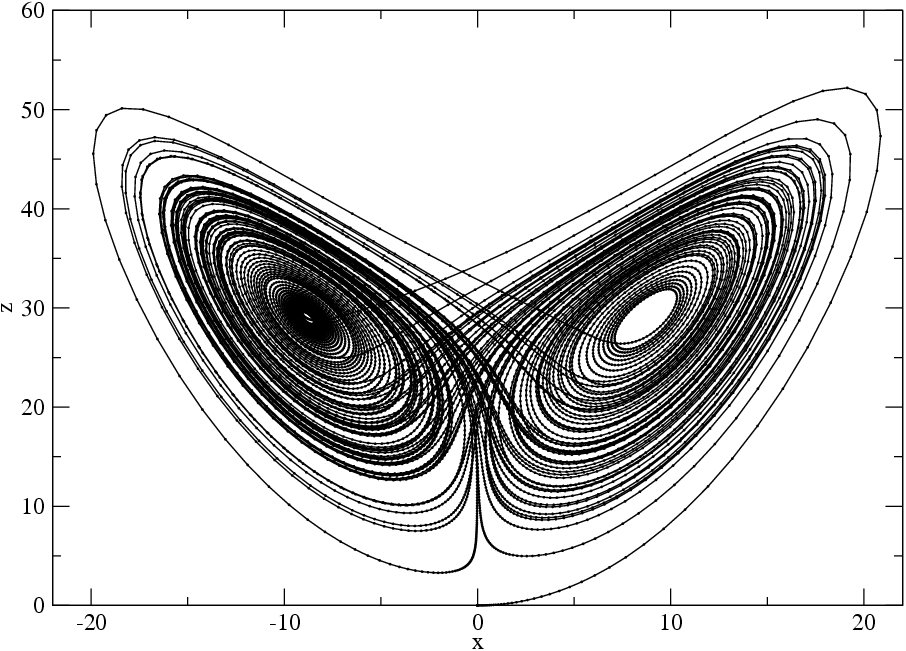
\includegraphics[scale=0.2]{/home/laboroco/vidaartificial/teoriacaos/images/lorenzatractor.jpg}
\caption{Atractor con dinámica caótica}
\label{atractor de lorenz}
\end{figure}
Eventualmente nosotros podriamos seleccionar las mejores orbitas de manera de obtener un mejor desempeño. Cada una de las orbitas que genera un atractor caótico es uno de los posibles caminos que el sistema puede tomar.
\subsection*{Función Logística}
Es una aplicación matemática que describe un modelo demográfico. Esta ecuación sencilla de grado dos, tiene como principal caracteristica su comportamiento caótico.
\begin{center}$x_{n+1}=rx_n(1-x_n)$\end{center}
donde $x_{n+1}$ es el sucesor resultante en función del valor anterior $x_n$ y el parametro de crecimiento $r$.
\begin{figure}[htp]
\centering
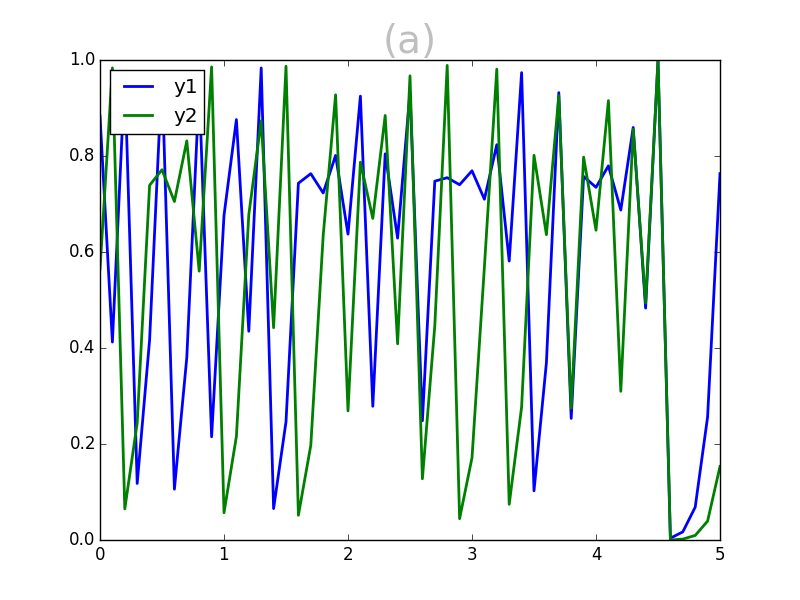
\includegraphics[scale=0.4]{/home/laboroco/vidaartificial/teoriacaos/caos.png}
\caption{Función Logistica asociada a dos parámetros distintos}
\label{}
\end{figure}
Si variamos el parámetro $r$ en el ragno [1.0 , 4.0] evaluando la función logística para cada una de estas constantes, se genera lo que se conoce como un \emph{diagrama de bifurcación}.
\begin{figure}[htp]
\centering
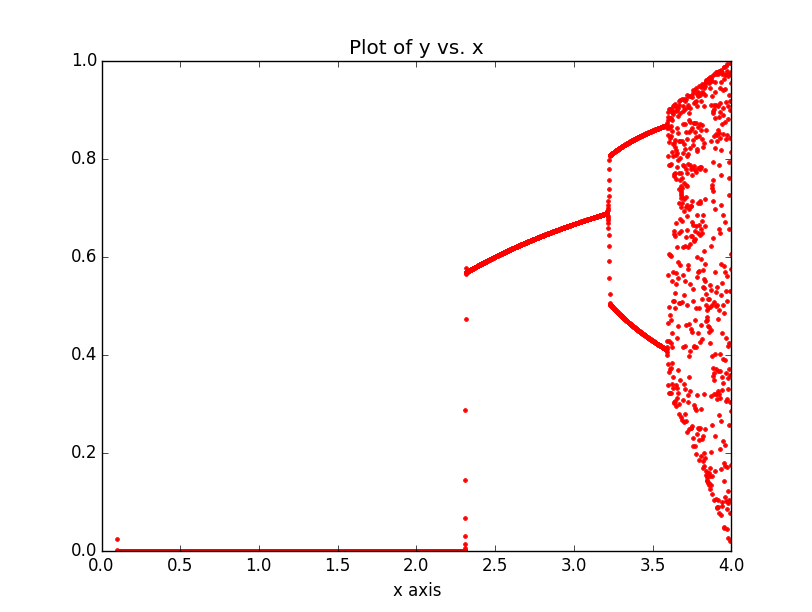
\includegraphics[scale=0.4]{/home/laboroco/vidaartificial/teoriacaos/images/bifurcacion.png}
\caption{bifurcación}
\label{}
\end{figure}
Note que a una tasa de crecimiento aproximadamente menor que 3.2 el cre-cimiento de una población se mantiene constante. En el primer intervalo [0 , 2.4[ tiende a cero, sin embargo desde el 3.5 notamos el comportamiento caótico; entre un valor y otro se producen variaciones significativas en cuanto a la distancia entre dos puntos.
\subsection*{Comportamiento Bacteriano}
Las bacterias heredan copias idénticas de genes, es decir, son clones. Sin embargo pueden evolucionar mediante cambios en el ADN. Cada bacteria tiene asociado un plasmido que es un fragmento de ADN (y el ADN propiamente tal).
Las bacterias pueden traspasar su material genético mediante tres formas:
\begin{enumerate}
\item Transformación
\item Transducción
\item Conjugación Bacteriana
\end{enumerate}
En ésta etapa de nuestra investigación hemos implementado la conjugación y transformación como método de traspaso de ADN. No consideramos plásmidos.
\begin{figure}[htp]
\centering
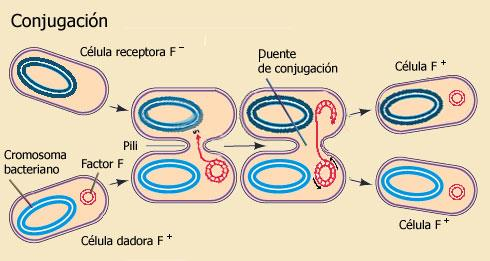
\includegraphics[scale=0.40]{1.png}
\caption{conjugación}
\label{con}
\end{figure}

\subsection*{Clasificación, Transformación, Mutación y Antibiótico}
Para definir la variabilidad/diversidad y la evolución de la población bacteriana utilizamos lo siguientes métodos:\\\\\textbf{Clasificación: }La clasificación biológica es la taxonomía (del griego taxis, que puede traducirse como "ordenamiento", y nomos, "regla"). En su significado más amplio, se trata de la ciencia dedicada a la clasificación que ordena a los diversos organismos dentro de una estructura o de un sistema.\\\textbf{Transformación:} 


%----------------------------------------------------------------------------------------
%	DESCRIPCION DEL PROBLEMA
%----------------------------------------------------------------------------------------
\section*{Descripción del Problema}
A partir de una población de bacterias optimizar el problema de XXXX. Cada organismo tiene un material genético (posible solución al problema) asociado a él. Las bacterias respetan ciertas reglas básicas que les permiten subsistir, tales como:
\begin{itemize}
\item Al encontrarse con otra bacteria dentro de su vecindad (von neumann) estas comparan su material genético y quien gane obtiene el ADN (solución) del oponente.
\item Si hay más de cuatro vecinos o en su defecto, ningúno, entonces la  bacteria muere en soledad.
\item Si hay un espacio vacío entre tres bacterias entonces nace un nuevo organismo
\item Las bacterias viven mientras exista un porcentaje deseado de organismos vivos.
\end{itemize}
Bajo estas condiciones se compararán los resultados de una población que obedece la teoria del caos y otra sin uso de este método.
%----------------------------------------------------------------------------------------
%	DESARROLLO DEL PROBLEMA
%----------------------------------------------------------------------------------------
\section*{Desarrollo del problema}
La población se representa a través de una matriz de dimensiones iniciales $NxN$ donde cada celda representa una bacteria. El ADN asociado a un organismo es un conjunto de números (arreglo) aleatorios.

%----------------------------------------------------------------------------------------
%	REFERENCE LIST
%----------------------------------------------------------------------------------------

\begin{thebibliography}{99} % Bibliography - this is intentionally simple in this template

\bibitem[Ott, Grebogi and Yorke, 1990]{Ott:1990dg}
\newblock "Controlling Chaos" Volume 64, Number 11 Physical Review Letters
\newblock  Pages 1196-1199

\bibitem[R.Contreras, M.A. Pinninghoff, R.Contreras, 2015]{Ott:1990dg}
\newblock "A new genetic algorithm approach: Is it a good
idea to deal with chaos theory in optimization
problems?"
  
\bibitem[James T. Townsend]{Ott:1990dg}
\newblock \emph{Chaos theory: A Brief Tutorial and Discussion} Indiana University

\bibitem[Étienne Ghys, 2012]{Ott:1990dg}
\newblock \emph{The Butterfly Effect} $12^{th}$ International Congress on Mathematical Education
COEX, Seoul, Korea
 
\bibitem[Geoff Boeing, 2015]{Ott:1990dg}
\newblock \emph{Chaos Theory and the Logistic Map} - PhD candidate, urban planning at UC Berkeley
\end{thebibliography}

%----------------------------------------------------------------------------------------

\end{document}